\documentclass[12pt,
article,
type=sta, %sta, diplom, bsc, pp, msc, dr, drfinal, sem, prosem
colorbacktitle,
instlogo,
accentcolor=tud1c,
oneside
]{tudthesis}

\usepackage[ngerman]{babel}
%\usepackage[english]{babel}

\usepackage[utf8]{inputenc}
%\usepackage[latin1]{inputenc}
%\usepackage[applemac]{inputenc}

% linebreak for urls in bitex
\usepackage{url}
\urlstyle{rm}

%listings
\usepackage{listings}
\lstset{language=C++}

\newcommand{\getmydate}{%
\iflanguage{ngerman}{%
  \ifcase\month%
    \or Januar\or Februar\or M\"arz%
    \or April\or Mai\or Juni\or Juli%
    \or August\or September\or Oktober%
    \or November\or Dezember%
  \fi\ \number\year%
}%
\iflanguage{english}{%
  \ifcase\month%
    \or January\or February\or March%
    \or April\or May\or June\or July%
    \or August\or September\or October%
    \or November\or December%
  \fi\ \number\year%
}
}
% changed counter for section wise counting
\usepackage{chngcntr}
\counterwithin{figure}{section} 
\counterwithin{table}{section} 

%user packages
\usepackage{todonotes}
\newcommand{\code}[1]{\texttt{#1}}
\newcommand{\tod}[1]{\todo[inline]{#1}}
\usepackage{hyperref}
\usepackage{graphicx}
\usepackage{caption}
\usepackage{subcaption}
\usepackage{float}
\usepackage{tabularx}
 
\setinstitutionlogo[height]{logo/ESlogo.png}

\begin{document}
\counterwithin{lstlisting}{section}
  \thesistitle{Projektseminar Echtzeitsysteme\linebreak[1]AUDO - Autonomous Unmanned Driving Unit}%
    {}
  \author{Nikolas Ziegelmayer, Nils Wittig, Fabian Burger, Ramona Volz und Maike Latsch}
  %do not add your student id!
  %\studentidx{1145456}
\thesisnumber{}
  \referee{}{Institut f\"ur Datentechnik\textbar Fachgebiet Echtzeitsysteme}
	
  \iflanguage{english}{
		\department{	\mbox{Department of Electrical Engineering}\\ and Information Technology (FB18)\\\\Adjunct Member Department of\\ Computer Science (FB20)\\\\Prof. Dr. rer. nat. A. Sch"urr\\\ Merckstra"se 25\\64283 Darmstadt\\\\www.es.tu-darmstadt.de}
		\group{Real-Time Systems Lab}
	}{
		\department{Elektrotechnik und \\Informationstechnik (FB18)\\\\Zweitmitglied Informatik (FB20)\\\\Prof. Dr. rer. nat. A. Sch"urr\\\ Merckstra"se 25\\64283 Darmstadt\\\\www.es.tu-darmstadt.de}
		\group{Fachgebiet Echtzeitsysteme}
	}
  
  \dateofsubmit{\today}
  \makethesistitle
  \affidavit{N. Ziegelmayer, N. Wittig, F. Burger, R. Volz, M. Latsch}
	
%	\cleardoublepage
%	\begin {abstract}
%	...
%	\end{abstract} 
	

	\pagenumbering{roman}
	\addtocontents{Anhang}{}
	\tableofcontents
	\clearpage
	\listoffigures
	\listoftables
	\clearpage
	
	\pagenumbering{arabic}
	\section{Einleitung}
\label{cha:einleitung}
Im Gegensatz zu den vergangenen Jahren war es die Aufgabe dieses Projektseminars Echtzeitsysteme eine Steuerung zu entwickeln, welche einen vorgegebenen Rundkurs durch eine Kamera erkennt und diesen absolvieren kann. In den letzten Jahren wurden Sensoren und die Abstände zu Wänden dafür genutzt. Durch eine Kamera und verschiedene Sensoren wird die Umgebung analysiert und durch Filterung und Regelung umgewandelt, um das Fahrzeug zu steuern. 
Die finale Implementation lässt das Fahrzeug autonom den Rundkurs bewältigen ohne dabei über die markierten Linien zu fahren. Als zweite Aufgabe wurde Hinderniserkennung mit Spurwechsel gewählt, hier erkennt das Fahrzeug ein Hindernis und wechselt die Spur, um diesem auszuweichen. Sollte die Strecke komplett blockiert sein oder das Fahrzeug sich auf eine reale Wand zu bewegen, wird dies erkannt und das Fahrzeug hält an. \\
In den folgenden Kapiteln werden die Grundlage der Hardware und Software, die Organisation des Teams, die Implementierung der Aufgaben und die Probleme beschrieben. Es wird auf die einzelnen Bestandteile der Regelung und der Bildverarbeitung eingegangen und der Entwicklungsprozess beschrieben. 

%%%%%%%%%%%%%%%%%%%%%%%%%%%%%%%%%%%%%%%%%%%%%%%%%%%%%%%%%%%%%%%%%%%%%%%%%%%%%%%%%%%%%%%%%%%%
\clearpage
\section{Grundlagen}
\label{cha:grundlagen}
In diesem Kapitel werden die verschiedenen Grundlagen auf der Hardware- und Softwareseite beschrieben. Dies schließt Informationen über das Modellauto, die verwendeten Kameras, das Metabetriebssystem ROS, OpenCV, die vorgegebenen Packages von PSES und die Gestaltung des Rundkursen in den Veranstaltungsräumen mit ein.

\subsection{Hardware}
\label{sec:hardware}
Die benötigte Hardware für das Projektseminar wurde allen Gruppen zur Verfügung gestellt und es gab eine kurze Einführung in die Arbeitsräume und den Umgang mit den einzelnen Teilen. Zur Verfügung standen das Modellfahrzeug, eine Kinect Kamera, eine Weitwinkelkamera, passende Akkus und Ladestationen und einiges an Klebeband. In den folgenden Unterabschnitten werden das Modellfahrzeug und die Kameras genauer beschrieben. 
\subsubsection{Modellauto}
\label{sec:modellauto}
Das zur Verfügung gesellte Fahrzeug ist einem Auto ähnlich. Es wurde speziell für das Projektseminar entwickelt und durch die TU Darmstadt gepflegt. Es besitzt vier Räder einen Motor und ist mit verschiedenen Sensoren, einer Kamera einem Mini-Computer und Mikrocontrollern ausgestattet. Da sich die Aufgabenstellung dieses Seminars auf Bildverarbeitung fokussierte, wird hier nicht näher auf die anderen Sensoren eingegangen. 
Die Steuerung erfolgt über den Computer, auf welchem ROS läuft (siehe \autoref{sec:ros}). Das Fahrzeug besitzt einen maximalen Lenkwinkel und eine maximale Geschwindigkeit, diese wurden durch eine bereitgestellte Fernsteuerung gemessen.
Das Mainboard ist mit diversen Anschlüssen ausgestattet, die es erlauben eine Tastatur, Maus und einen Bildschirm anzuschließen. Des Weiteren ist eine Kinect und eine Weitwinkelkamera vorhanden (siehe \autoref{sec:kameras}). Die Stromversorgung während der Fahrt übernehmen zwei Akkupacks.
\tod{Bild Auto}
\subsubsection{Kameras}
\label{sec:kameras}
Zu Beginn war eine Kinect Kamera auf dem Fahrzeug verbaut. Diese wurde in den frühen Phasen der Entwicklung genutzt, jedoch kurz nach der Zwischenpräsentation durch die Weitwinkelkamera ersetzt. Diese zeichnet sich durch ein 120° Sichtfeld, eine FullHD Auflösung und einem leicht einstellbaren Positionswinkel aus.
Grund dafür war eine schlechte Farbwahrnehmung der Kinect, diese wurden übersaturiert dargestellt (näheres siehe \autoref{sec:sichtfeld}). Eine Erkennung der richtigen Farbe durch die bereitgestellten Bibliotheken war dadurch nicht mehr möglich. 
Mit der Weitwinkelkamera wurde dieses Problem gelöst. Die Farben wirken natürlicher und sind durch die angewendeten Filtermethoden extrahierbar. Da die Halterung der Webcam auf Computerbildschirme ausgerichtet ist, musste eine elegante Lösung gefunden werden. Ein festkleben mit Klebeband hielt für den Anfang, war jedoch zu anfällig für ein Verstellen der Kamera.
Deswegen  wurde ein 3D-Modell entwickelt und eine passende Halterung im Fablab\footnote{https://www.fablab.tu-darmstadt.de/} gedruckt. Mit dieser konnte die Kamera stabil am Fahrzeug befestigt werden und es gab keine Schwankungen mehr durch andere Kamerapositionen (nähere Informationen in \autoref{sec:befestigung}). 
\begin{figure}
	\centering
	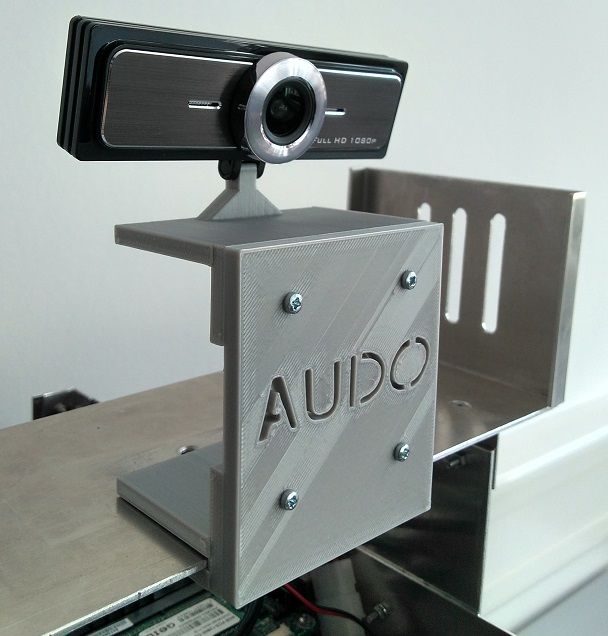
\includegraphics[width=0.5\textwidth]{images/Foto_Halterung.jpg}
	\caption{Halterung der Weitwinkelkamera}
	\label{abb:halterung}
\end{figure}
\tod{Bild updaten}
%%%%%%%%%%%%%%%%%%%%%%%%%%%%%%%%%%%%%%%%%%%%%%%%%%%%%%%%%%%%%%%%%%%%%%%%%%%%%%%%%%%%%%%%%%%%%
\subsection{Software}
\label{sec:software}
In diesem Abschnitt wird die Software vorgestellt, die auf dem Mini-Computer läuft und während der Programmierung genutzt wird. Das Hauptbetriebssystem stellt Lubuntu dar\footnote{https://lubuntu.net/}. Auf diesem ist das Metabetriebssystem ROS installiert, welches die eigentlichen Funktionen übernimmt. Die Programmierung der Nodes geschieht mit dem Programm RoboWare Studio, dort sind alle vorgefertigten Nodes und die selbst erstellten  übersichtlich dargestellt. Programmiert wird in der Programmiersprache C++. \\
Im folgenden werden häufig genutzte Pakete beschrieben und das Meta-Betriebssystem ROS.

\subsubsection{ROS - Robot Operating System}
\label{sec:ros}
ROS ist ein Metabetriebssystem für Roboter, welches auf Linux basiert und in vielen Unternehmen für Steuerung von Robotern genutzt wird. Es stellt mehrere Pakete zur Verfügung, die einige nützliche Funktionen ermöglichen. Dazu gehört die Verteilung auf mehrere Systeme im Netzwerk, Paketverarbeitung und die Kommunikation zwischen den Nodes \cite{einfuehrungROS}.
Die Kommunikation findet durch ein Publish-Subscribe-System statt. Die einzelnen Nodes publishen zu  bestimmten Themen Nachrichten, deren Inhalt sich auf das Thema bezieht. So erhält man zum Thema \code{/uc\_bridge/usr} über eine Subscription Nachrichten über die Werte des rechten Abstandssensors. Auch die Steuerung des Motors und des Lenkwinkels geschieht über das puplishen von Nachrichten. 
Die Eigenschaften der Pakete und Tutorials zu den Funktionen sind auf der Website von ROS zu finden und erleichtern den Einstieg. Durch Open Source lässt sich schnell herausfinden was wirklich benötigt wird und welche Funktionen im späteren Verlauf hilfreich sein könnten.

\subsubsection{OpenCV}
\label{sec:openCV}
Zur Verarbeitung der Kamerabilder wird die freie Bibliothek OpenCV\footnote{https://opencv.org/} genutzt, diese ist auch durch eine Node in ROS eingebunden und einfach nutzbar. Zur Verwendung wird das von der Kamera erhaltene Objekt in der Datenstruktur von OpenCV als \code{cv::Mat} gespeichert. Darauf lassen sich alle späteren Bearbeitungsschritte ausführen. 
Sie stellt viele nützliche Funktionen bereit, die das Erkennen der Fahrspuren und der Hindernisse erleichtern. Dazu gehören zum Beispiel \code{cv::wrapperperspective}, mit der das Bild in eine Bird Eye View umgewandelt wird und \code{cv::imshow} zum Anzeigen des aktuellen Bildes. Interessanterweise funktionierte diese Funktion nur, wenn sie im Zusammenhang mit \code{cv:waitKey} aufgerufen wurde. 
Mittels \code{cv::cvtColor}, \code{cv::inRange} und \code{cv::GaussianBlur} lässt sich der Farbraum des Originalbildes transformieren und in diesem anschließend alle Farben herausfiltern, die in einem bestimmten Bereich liegen. 
In der späteren Verarbeitung war es nötig Farbwerte von einzelnen Pixeln auszuwerten, dies geschah mit Hilfe der Methode \code{cv::mat.at<uchar>(y,x)}. Auch ein Einzeichnen von neuen Punkten war möglich und für die spätere Kurvenerkennung hilfreich. 

\subsubsection{PSES Packages}
\label{sec:psespackages}
Zur Kommunikation mit den einzelnen Fahrzeugteilen sind von den Veranstaltern einige Nodes vorgegeben, dazu gehören \code{pses\_uc\_bridge}, \code{pses\_simulation}, \code{pses\_dashboard} und \code{pses\_odometry}. Von diesen wurde in der finalen Lösung nur \code{pses\_uc\_bridge} genutzt. Diese Node muss zuerst gestartet werden, da sie alle Steuerfunktionen übernimmt und die Publish- und Subscribe-Komponenten für die verschiedenen Werte erstellt. 
Über \code{pses\_dashboard} kann das Fahrzeug manuell gesteuert werden, dies wurde genutzt, um herauszufinden wie groß der maximale Lenkwinkel und die Geschwindigkeit waren, die das Fahrzeug bewältigen kann. Da diese Node gestartet über eine graphische Oberfläche verfügt, war auch ein Ablesen der jeweiligen Sensorwerte möglich. \code{pses\_simulation} stellt eine Simulationsumgebung für das Fahrzeug da, in der der erstellte Code getestet werden konnte. Dies wurde jedoch nicht genutzt, da ein Testen in der realen Umgebung bessere Werte lieferte und in der Simulation kein Kamerabild simuliert werden konnte. 
Die Node \code{pses\_odometry} dient zur Selbstlokalisierung des Fahrzeuges. Nach dem Start ist es möglich die zurückgelegte Strecke und die einzelnen Positionsdatenveränderungen zu berechnen, um sich ein genaueres Bild über die Position des Fahrzeuges in seiner Umwelt zu machen.

%%%%%%%%%%%%%%%%%%%%%%%%%%%%%%%%%%%%%%%%%%%%%%%%%%%%%%%%%%%%%%%%%%%%%%%%%%%%%%%%%%%%%%%%%%%%%%
\subsection{Rundkurs}
\label{sec:rundkurs}
Zur Verfügung standen zwei Räume in Gebäude S311, dort wurden die Fahrzeuge, die Akkus und alles weiter benötigte Material aufbewahrt. Zusätzlich boten sie Platz zum Programmieren und basteln und in einem Raum war der Boden mit einem Rundkurs ausgestattet. Dieser war mit farbigem Klebeband auf eine Teichfolie in mitten des Raumes geklebt. Er bot zwei grüne Linien am Rand und eine pinke Mittellinie. Hier fanden sich öfter mehr als eine Gruppe ein, um den zuvor programmierten Code zu testen, die Kameras einzustellen oder die Lenkwinkel zu messen. \\
Da dieser Rundkurs für die finale Bewertung und den Wettbewerb am Ende genutzt wird, konnte man seine Regelung und Steuerung anpassen und die Lichtverhältnisse konstant halten. Es wurde schnell klar, dass geringe Änderungen des Lichtes eine große Änderung bei der Farbwahrnehmung der Kamera nach sich zogen. 

	\clearpage
	\chapter{Organisation}
\label{cha:Organisation}
In diesem Abschnitt wird das Projektmanagment des Teams beschrieben, das zum erfolgreichen Abschluss unseres Projektes beigetragen hat. Bei einem Team mit fünf Personen ist es wichtig Maßnahmen zur Dateiverwaltung und Organisation zu treffen, um eine gute Zusammenarbeit anzusteuern.

\section{Gruppentreffen und Organisation}
\label{sec:gruppentreffenundorganisation}
\subsection*{Gruppentreffen}
Wir entschieden uns bei unserem ersten Teamtreffen für eine Versionsverwaltung und eine Organisationsplattform und richteten diese zusammen ein.

Im zwei Wochen Takt traf sich vorzugsweise das gesamte Team mit einem Betreuer des Projektes. Mit ihm besprachen wir den aktuellen Stand unseres Projektes und gegebenfalls Probleme im Team. Diese Treffen waren organisatorischen Zwecken gewittmet, es wurden keine Fragen direkt zur Implementierung geklärt. Als das Projekt grundlegend funktionierte, wurden Anregungen zur Erweiterung der Aufgabenstellung gegeben. 

Zur Besprechung von Regelungs- und Implementierungsfragen, gab es annähernd jede zweite Wochen ein Regelungstechniktreffen, bei dem sich zwei Teammitglieder jeder Gruppe einfunden. Es wurde der Stand der jeweiligen Gruppen untereinander ausgetauscht und Fragen diskutiert. Für weitere Fragen und Anregungen stand dort ein Betreuer der Regelungstechnik zur Verfügung.

Zusätzlich zu den Beratungsgesprächen legten wir feste wöchentliche Treffen mit allen Gruppenmitgliedern fest. Jeder berichtete von seinem Vorgehen der vergangenen Woche, so dass alle im Team den Überblick über den aktuellen Stand des Projektes hatten. Daraufhin wurden Ideen und Anregungen zusammengetragen und die Planung für die nächste Woche erarbeitet. Mit Hilfe der im Folgenden noch erwähnten Organisationsplattform Trello wurden die Aufgaben erfasst und den interessierten Gruppenmitgliedern zugeordnet. 

\subsection*{Team}

Wir entschieden die Zeitplanung dinamisch zu halten, da es schwer einschätzbar ist, wie viel Zeit eine einzelne Aufgabe in Anspruch nimmt. Erfahrungen aus anderen Projekten haben gezeigt, dass dieses Vorgehen sinnvoll ist. Wir setzten uns als Ziel, dass nach \nicefrac{2}{3} der Projektzeit eine funktionierende Version vorhanden ist, um genügend Zeit für die Optimierung und Dokumentation einzuplanen und gegebenenfalls einen ausreichenden Zeitpuffer zur Verfügung zu haben. Jede Woche bei dem Gruppentreffen wurde festgelegt, wer sich welcher neuen Aufgabe annimmt und wir schätzten erneut ab, wie viel Zeit eine angefangegne Aufgabe noch benötigen wird.


Nachdem sich alle in die Dokumentation eingelesen hatten, erarbeiteten wir erste Grundlagen zusammen, damit jeder ein Grundwissen über das Modellauto hatte. Es bildeten sich Aufgabengruppen für Organisation, Regelung und Bildverarbeitung, diese wurden weitgehendst parallel behandelt. Die Verantwortung für diese Teilgruppen wurde auf die Mitwirkenden aufgeteilt. Jedes Gruppenmitglied konnte bei jeder Aufgabengruppe helfen, allerdings ist es wichtig Verantwortliche festzulegen, um den Überblick zu bewahren und Zielführend zu agieren. Als die Tests der Bildverarbeitung und Regelung die aufgestellten Bedingungen erfüllten, schlossen wir diese Aufgabenbereiche zusammen und erlangten dadurch das Fahren durch den Rundkurs. Neben der Optimierung des Rundkurses wendete sich eine Subgruppe dem zweiten Thema, Hinderniserkennung mit Spurwechsel, zu.

Es gab viele Aufgaben, die direkt am Fahrzeug getestet werden mussten. Da das gleichzeitige Testen mehrerer Aufgaben meist nicht möglich war, unterstützte man beim Zusammenkommen die anderen Teammitgliedern über die Aufgabenverteilung hinaus. Jeder teilte sich seine Zeit selbstständig jede Woche ein. Wir kommunizierten, welche Aufgabe wann bearbeitet wird, damit Interessengruppen zusammenfinden konnten. 

\section{Aufgabenverwaltung}
\label{sec:aufgabenverwaltung}


\section{Versionsverwaltung}
\label{sec:versionsverwaltung}

	\clearpage
	\chapter{Implementierung}
\label{cha:Implementierung}
\section{Bildverarbeitung und Erkennung von Fahrspuren}
\label{sec:spurerkennung}

TODO: Fabian

\section{Erkennung von Kurven und Geraden}
\label{sec:kurvenerkennung}

TODO: Fabian

\section{Erkennung von Hindernissen}
\label{sec:hinderniserkennung}

TODO: Fabian

\section{Kollisionsvermeidung}
\label{sec:kollision}

Um in allen Fahrsituationen eine Beschädigung des Fahrzeugs zu vermeiden, wird eine Kollisionsvermeidung eingesetzt. Diese verhindert unabhängig von Fahrspuren oder erkannten Hindernissen, dass es im Fahrbetrieb zu einem Zusammenstoß mit anderen Gegenständen oder der Wand kommt. Hierzu werden die Daten des vorderen Ultraschallsensors ausgewertet, der einen ungefähren Abstandswert zum nächstgelegenen Gegenstand liefert.

Um aus dem fehlerbehafteten Signal verwertbare Daten zu erhalten werden die Werte des Sensors geglättet. Dies geschieht indem die letzten 20 Sensorwerte gemittelt werden. Liegt der Durchschnitt unter einem Schwellwert, wird der Motor angehalten. Als praxistauglicher Wert hat sich 0.35 erwiesen, also ein Abstand von 35 Zentimetern.

Ein besonderes Problem ergibt sich aus der Tatsache, dass die Werte des Sensors in unregelmäßigen Abständen kurzzeitig auf den Wert Null springen. Dies entspräche einem Gegenstand direkt vor dem Sensor, was schon alleine aufgrund der Fahrzeuggeometrie nicht plausibel ist. Diese Werte müssen daher von der Auswertung ausgenommen werden.

(Codeausschnitt: collision_protection())
(Bild des Ultraschallsensors)

\section{Regelungskonzept und Spurhaltung}
\label{sec:wallfollower}

Nach umfangreichen Tests zu Beginn des Projekts wurde ein strukturvariabler Regelungsansatz mit PD-Reglern gewählt. Eine strukturvariable Regelung lässt sich vor Allem dann sinnvoll einsetzen, wenn zwischen wenigen bekannten Arbeitspunkten umgeschaltet werden muss. Die Rennstrecke des Projektseminars Echtzeitsysteme lässt sich Kurven- und Geradenabschnitte aufteilen. Aufgrund der hohen Nichtlinearität der Lenkungsmechanik (insbesondere Lose, Haftreibung, Gleitreibung) lässt sich mit einem einzigen PD-Regler kein zufriedenstellendes Regelverhalten in allen Fahrsituationen erzielen. Eine stationäre Genauigkeit ist in diesem Fall zur Spurhaltung im Übrigen nicht erforderlich, solange die bleibende Regelabweichung in der Praxis so klein ist, dass alle Fahrsituationen der Rennstrecke ohne Linienüberschreitung gefahren werden können. Mit einem gut eingestellten PD-Regler lässt sich diese Anforderung erfüllen.

Die Bildverarbeitung liefert die Positionsdaten aller Markierungslinien, die im Bildausschnitt der Kamera erfasst werden. Da die Position der Kamera auf dem Fahrzeug sich nicht ändert, kann ein fester Sollwert für den Abstand zu diesen Linien vorgegeben werden. Es muss zur Berechnung der Regelabweichung lediglich bekannt sein, ob das Fahrzeug sich an der rechten oder an der linken Fahrbahnbegrenzung orientieren soll. Näheres hierzu in Abschnitt \ref{sec:fahrsituationen}.


\section{Implementierung des PD-Reglers}
\label{sec:pdregler}

Die Berechnung der Lenkwinkelregelung erfolgt in mehreren Schritten. Zunächst wird aus den situationsabhängigen Reglerparametern sowie Führungsgröße und aktueller Position eine Stellgröße berechnet. Der differentielle Anteil des PD-Reglers greift hierbei auf den aktuellen und vorherigen Wert der Regelabweichung, sowie die verstrichene Zeitdauer seit der letzten Berechnung zu.

Codeausschnitt: PD Regler

Anschließend erfolgt eine Begrenzung der Stellgröße. Die Hardware erlaubt Lenkwinkel im Bereich -800....+800. Um Beschädigungen zu vermeiden wird der maximale Lenkwinkel softwareseitig auf -700....+700 begrenzt. Bei höheren Werten kommt es zu einem Blockieren des Lenkgetriebes.

Um ein ruhiges Lenkverhalten zu erreichen werden die Ausgangswerte des Reglers zum Schluss geglättet. Dazu wird ein gewichteter Mittelwert der letzten Stellgrößen gebildet. Die Gewichtung erfolgt in Abhängigkeit des zeitlichen Verlaufs. Dabei hat der zuletzt berechnete Wert das größte Gewicht, ein 0,3 Sekunden zurückliegender Wert hingegen nur das halbe Gewicht. Der gewichtete Mittelwert erzeugt ein ruhiges Regelverhalten, ohne jedoch die Regelung zu stark zu verzögern.

Codeausschnitt: Regler Glättung

\section{Implementierung verschiedener Fahrsituationen}
\label{sec:fahrsituationen}

Das Konzept sieht die Aufteilung der zu fahrenden Strecke in vier wiederkehrende Fahrsituationen vor:

(Aufzählung: Geradeausfahrt, Kurvenfahrt, Übergang von Geraden- zu Kurvenfahrt, Übergang von Kurven- zu Geradenfahrt)

Je nach Situation wird zwischen einem Regler für Geradeausfahrt und einem Regler für Kurvenfahrt umgeschaltet. Die Übergangszustände dienen lediglich der stufenweisen Geschwindigkeitsanpassung beim Wechsel zwischen den beiden Streckenabschnitten. Die Umschaltung zwischen den verschiedenen Reglern erfolgt in Abhängigkeit vom gewählten Fahrmodus (siehe Abschnitt \ref{sec:fahrmodi}).

Der Regler für die Geradeausfahrt zeichnet sich durch (.....) aus, während der Regler für die Kurvenabschnitte (.....).


\section{Einleitung eines Spurwechsels}
\label{sec:spurwechsel}

Die Implementierung eines Spurwechsels eröffnet vielfältige Möglichkeiten. Während ein Spurwechsel auf geraden Abschnitten der Strecke unproblematisch ist, kann es im Zusammenhang mit Kurven zu Problemen kommen. Wird eine Kurve auf der äußeren Spur durchfahren, so ist während der Kurvenfahrt grundsätzlich kein Wechsel auf die innere Spur möglich. Die konstruktive Begrenzung des Lenkwinkels wird durch die Kurvenfahrt schon komplett ausgenutzt, sodass kein Spielraum für ein Ausweichen nach innen mehr bleibt. Weniger problematisch ist das Ausweichen von der inneren auf die äußere Spur während einer Kurvenfahrt.

Auf der Rennstrecke des Projektseminars gibt es nur zwei Varianten eines Spurwechsels: von der rechten auf die linke Spur, und von der linken auf die rechte Spur. Grundsätzlich können diese Wechsel vorgenommen werden, indem der Regler-Sollwert auf den jeweils anderen Fahrbahnrand gesetzt wird. Dazu muss jedoch zunächst sichergestellt werden, dass sich überhaupt beide Fahrbahnmarkierungen im Sichtfeld der Kamera befinden. Daher wird (....)


\section{Fahrmodi und Wettbewerb}
\label{sec:fahrmodi}

Im Rahmen dieses Projektseminars sind zwei Aufgaben zu erfüllen: das Absolvieren einer kompletten Runde in möglichst geringer Zeit, und die Hinderniserkennung mit Spurwechsel bei möglichst wenigen Linienübertritten. Um beide Aufgaben möglichst gut zu lösen werden zwei verschiedene Fahrmodi implementiert, die sich durch die Fahrgeschwindigkeit und die Kriterien zur Wahl der Fahrspur unterscheiden.

\subsection{Fahrmodus 1: Rundenzeit}

tbd

Im ersten Fahrmodus liegt die Herausforderung in der Minimierung der Rundenzeiten. In diesem Modus wird ohne Hindernisse auf der Strecke gefahren, daher ist die Hinderniserkennung abgeschaltet. 

\subsection{Fahrmodus 2: Hinderniserkennung und Spurwechsel}

In diesem Modus spielt die Fahrgeschwindigkeit eine untergeordnete Rolle, weshalb sie auf einen konstanten und relativ niedrigen Wert gesetzt wird. Zunächst orientiert sich das Fahrzeug am rechten oder linken Fahrbahnrand und folgt der Spur. Solange sich kein Hindernis auf der Strecke befindet, wird dieser Zustand beibehalten. 

Ein Spurwechsel setzt voraus, dass dem Fahrzeug die eigene Position auf der Fahrbahn bekannt ist. Da dem Fahrzeug vorgegeben wird auf welcher Fahrspur es fahren soll, und die Regler ein schnelles Regelverhalten besitzen, kann im Allgemeinen davon ausgegangen werden, dass sich das Fahrzeug auf der vorgegebenen Fahrspur befindet.

Sobald ein Hindernis in das Sichtfeld der Kamera eintritt liefert die Bildverarbeitung dessen Koordinaten. Da auch die Koordinaten der beiden Fahrspuren bekannt sind, kann aus den Daten ermittelt werden, ob sich das Hindernis auf der aktuellen Fahrspur des Autos befindet. Befindet sich das Hindernis auf der eigenen Fahrspur, wird rechtzeitig ein Spurwechsel veranlasst. Andernfalls wird das Hindernis ignoriert und die Fahrt fortgesetzt.

Der Spurwechsel wird durch die Erkennung eines Hindernisses eingeleitet. Die Bildverarbeitung liefert dabei die Positionen des rechten und linken Randes eines Hindernisses, sodass neben der Position auch dessen Breite bekannt ist (siehe \ref{sec:hinderniserkennung}). Für den Spurwechsel entscheidend ist die Frage, ob sich das erkannte Hindernis überhaupt auf der gleichen Fahrspur wie das Fahrzeug befindet. Ist das nicht der Fall, stellt es kein Hindernis dar und kann ignoriert werden.

Codeausschnitt: Hinderniserkennung


	\clearpage
	\chapter{Probleme}
\label{cha:Probleme}

\section{Kinect - unnatürliche Farben}
\label{sec:farben}
Die Kamera der Kinect hat eine unnatürliche Farbdarstellung.
Es sind sind starke Unterschiede zwischen Kamerabild und der Wirklichkeit zur erkennen.
\\
TODO: Zeige ein Bild der Kinect und ein Bild der Webcam
\\
Die Farben der Kinect sind übersaturiert und haben teilweise nicht einmal den richtigen Farbton.

\section{Kinect - kleines Sichtfeld}
\label{sec:sichtfeld}
Das Sichtfeld der Kinect Kamera fällt relativ klein aus.
Das hat auch damit zu tun, dass die Kinect in einem Winkel auf dem Fahrzeug angebracht ist, mit dem das Sichtfeld erst circa 30cm vom Fahrzeug entfernt beginnt.
Dadurch kann der Abstand des Fahrzeuges zur Fahrbahnbegrenzung zum aktuellen Zeitpunkt nicht ohne weiteres bestimmt werden. 
Zudem ist die Kamera in der Kinect am rechten Rand platziert.
Dadurch ist die linke Fahrbahnbegrenzung häufig nicht im Sichtfeld.
Dieser Effekt wird noch durch die Transformation zum Bird-Eye View verstärkt.
\\
TODO: Vllt Bild von Webcam und Kinect zum Vergleich der Sichtfelder
\\
Um eine robuste Fahrbahnerkennung zu implemetieren, sind ordentliche Ausgangsdaten von großer Wichtigkeit.
In unserem Fall benötigen wir eine natürliche Farbdarstellung, ein ausreichend großes Sichtfeld das möglichst nah am Fahrzeug beginnt und eine flüssige Bildrate. 
Alle diese Anforderungen werden von der Webcam erfüllt.
Die Webcam kann zudem sehr flexibel auf dem Fahrzeug angebracht werden.
\\
Die Halterung der Webcam verursacht allerdings ein weiteres Problem.
Die Webcam sakt durch Vibrationen die beim Fahren entstehen nach einiger Zeit etwas ab.
Das heißt die Webcam zeigt mehr in Richtung Boden.
Das hat merkliche Auswirkungen auf die Transformation zum Bird-Eye View.
Wenn der Bird-Eye View nicht mehr korrekt berechnet wird, funktioniert die Erkennung der Fahrsituation nicht mehr so gut.
Genauer wird nicht mehr erkannt, wann sich das Fahrzeug auf einer Geraden befindet.
Da die Regelung abhängig von der Fahrsituation ist, kann das Fahrverhalten schlechter werden.

\section{Webcam verändert Belichtung zur Laufzeit}
\label{sec:belichtung}
Die Webcam passt ihre Belichtung an die aktuellen Lichtverhältnisse zur Laufzeit an.
Das führt leider dazu, dass selbst kleine Veränderungen der Lichtverhältnisse die Belichtung ändern, wie zum Beispiel Lichtspiegelungen auf dem Boden.
Wenn sich die Belichtung ändert, ändern sich auch schlagartig die Farbwerte.
Um keine komplizierte Anpassung der Filterparameter während der Laufzeit vornehmen zu müssen, muss die Belichtung konstant gehalten werden.
Das ist bei dieser Webcam nicht in Software machbar.
Wir haben einen pragmatischen Ansatz gewählt um dieses Problem zu lösen.
Wir blenden die Webcam mit einer LED Leiste.
Die LED Leiste wird über das 12V Boardnetz gespeißt.
Damit nimmt die Webcam die Umgebung immer sehr hell wahr.
Leichte Veränderungen der tatsächlichen Lichtverhältnisse werden durch das Blenden einfach herausgefiltert. 
Das Ergebnis ist eine konstante Belichtung und somit auch konstante Farbwerte.

\section{Fahrwerk}
\label{sec:fahrwerk}
Die Räder kollidieren bei zu hohem Lenkwinkel mit dem Gehäuse.
Deswegen begrenzen wir den maximalen Lenkwinkel auf einen ausgemessenen Wert.
\\
Die Lenkmechanik des Fahrzeugs ist aus Plastik und nicht sonderlich genau gefertigt.
Das hat zur Folge, dass die Lenkung ein merkliches Spiel hat. 
Für uns bedeutet das, dass kleine Veränderungen am Lenkwinkel keine realen Auswirken haben. 
Außerdem liegt relativ viel Last auf der Vorderachse, weil der Laptop Akku und die Kinect vorne im Fahrzeug platziert sind.
Dadurch wird die Lenkmechanik noch zusätzlich belastet.
Bei höheren Geschwindigkeiten sollte sich dieser Effekt allerdings abschwächen. 
Durch diese Effekte können wir uns nicht darauf verlassen, dass nach dem Einstellen eines Lenkwinkels, dieser auch tatsächlich anliegt.
In der Praxis fahren wir allerdings immer mindestens so schnell, dass dieser Effekt keine allzu großen Auswirkungen hat.
\\
Ein weiteres Problem besteht darin, dass der Lenkwert der an die UC_Bridge gesendet wird, sich nicht linear in einen Lenkwinkel umrechnen lässt.
Die Beziehung zwischen Lenkwert und Lenkwinkel auszumessen gestaltet sich schwierig.
Da diese Beziehung stark von der Geschwindigkeit und der Last auf die Lenkmechanik abhängt.
Wenn der tatsächliche Lenkwinkel durch passende Sensoren regelmäßig gemessen werden würde, könnte man eine Regelung für den Lenkwinkel konzipieren.
Wir haben uns um dieses Problem nicht weiter gekümmert und haben uns stattdessen darauf konzentriert eine möglichst robuste Regelung zur Fahrspurhaltung zu implementieren.
Um die Lenkmechanik nicht unnötig zu belasten haben wir eine möglichst ruhige Regelung vorgenommen.






	\clearpage
  
	\bibliographystyle{alphadin}
	\bibliography{literature}
	
	\begin{appendix}
	\section{Anhang}
	\end{appendix}

\end{document}
